\chapter{Quantised vortices in droplets}
	One of the most unambiguous signatures of the quantum mechanical nature of a substance---and indeed superfluidity---is the appearance of quantised vortices. In contrast to a normal fluid, which will rotate as a solid body when its container moves at low angular velocity, a superfluid will remain at rest. However, above a certain critical angular velocity the thermodynamically stable state of a superfluid includes one or more quantum vortices. Such a vortex can be characterised by a macroscopic wave function and quantised velocity circulation in units of $\kappa=\frac{h}{m}$, where $h$ is Planck’s constant and $m$ is the mass of the $^4$He atom [2,3]. Recently, the study of vorticity was extended to finite systems such as BECs confined to traps [3,4]. The transfer of energy and angular momentum in finite systems between quantised vortices and surface excitations is of particular interest, as it defines the nucleation dynamics, shape, and stability of the involved vortices [3,4]. In comparison to confined BECs, $^4$He droplets are self-contained and present a case for the strongly interacting superfluid. Moreover, the diameter of a vortex core which is approximately 0.2 nm in superfluid $^4$He [2] is small relative to the droplet size, suggesting a three-dimensionality of the vortices in droplets. Vorticity in $^4$He droplets has therefore attracted considerable interest [5–8].\\
	
	A schematic of the experiment is shown in Fig. \ref{fig:vortex-machine}. Helium droplets are produced by expansion of He, at 20 bar and a temperature $T_0$=5.4--7 K, into vacuum through a nozzle of diameter D 1⁄4 5 "m. The droplets cool rapidly via evaporation and reach a temperature of 0.37 K [20], which is well below the superfluid transition temperature T! 1⁄4 2:17 K [2,3]. Further downstream, the droplets capture 103–106 Ag atoms in an oven [21]. The droplets are then collided against a thin carbon film substrate at room temperature [21]. Upon impact, the droplets evaporate, leaving on the surface the Ag traces, which are subsequently imaged via a transmission electron microscope (TEM).
	\begin{figure}[t]
		\begin{center}
			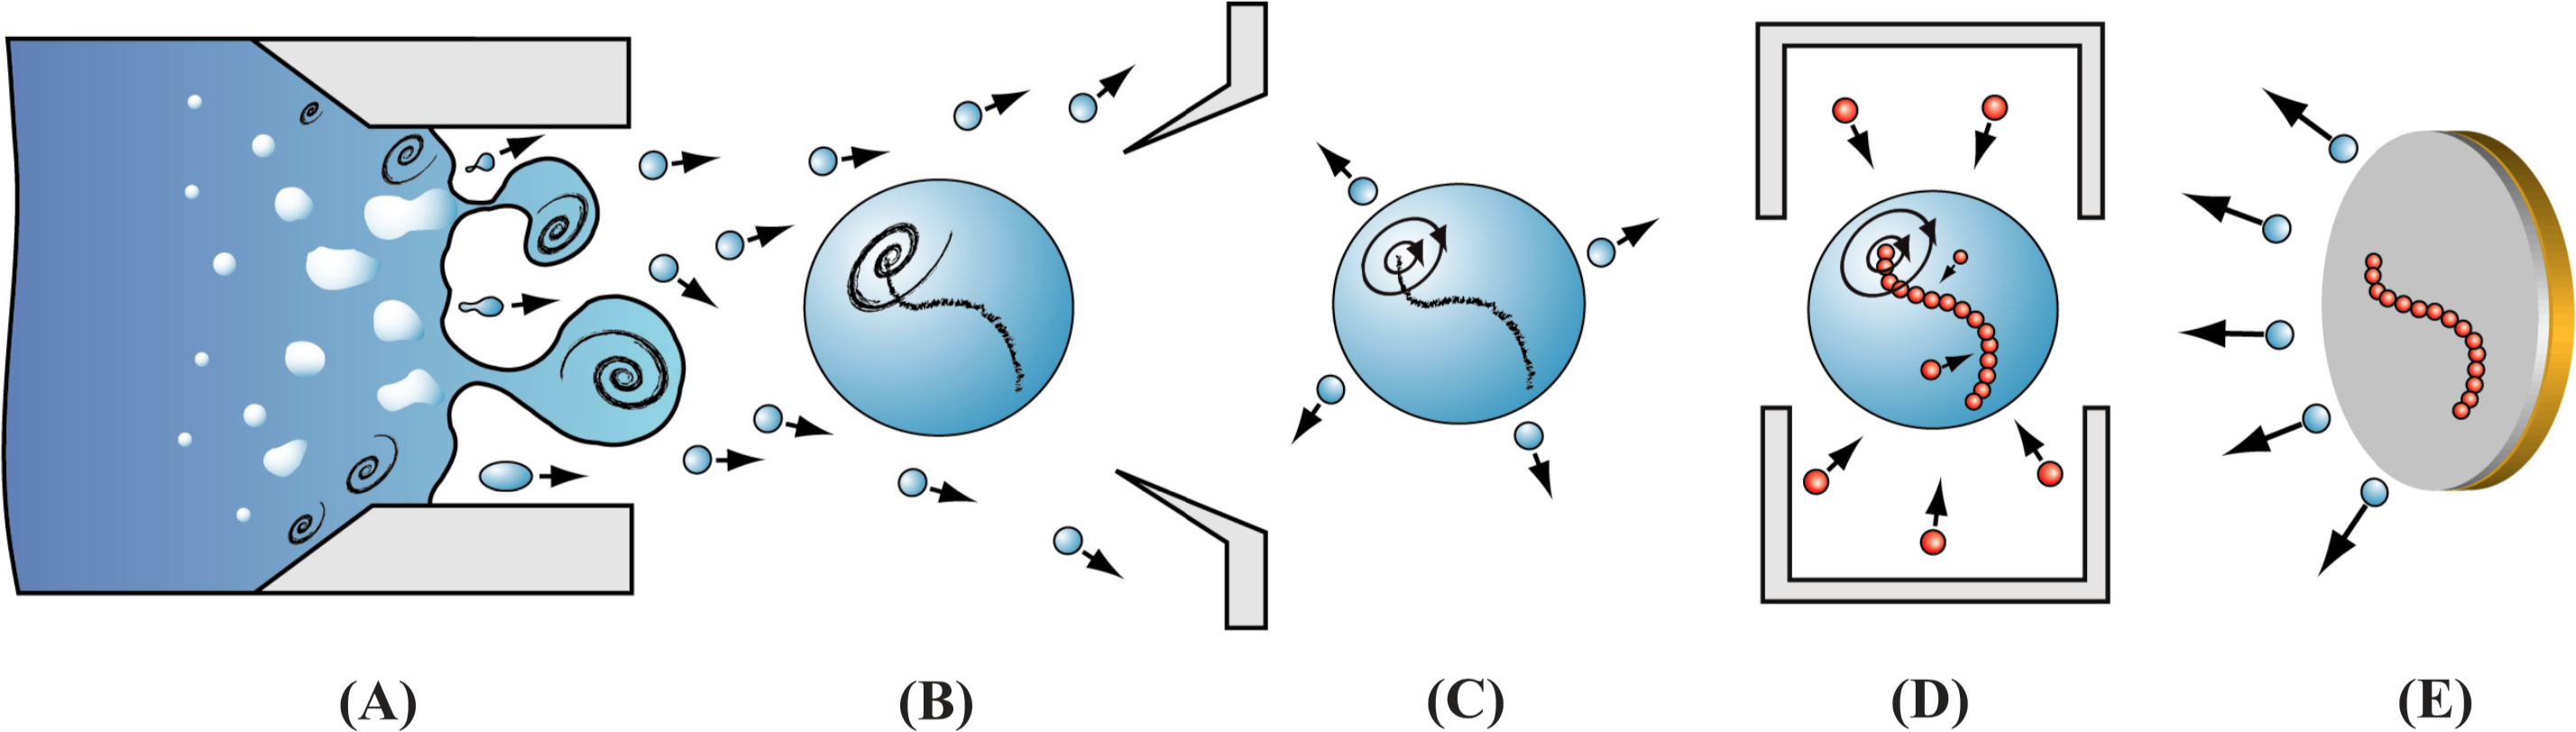
\includegraphics[width=\textwidth]{vortex-machine}
			\caption{Schematic of the experiment. (a) He fluid expands in vacuum and (b) breaks up into rotating droplets. (c) A quantum vortex is formed as a consequence of fast evaporative cooling of the droplet to below $T_\lambda$. (d) The droplet is doped with Ag atoms, which are attracted to the vortex core. (e) The droplet then collides with the carbon surface leaving behind the Ag trace, whereas the He evaporates.}
			\label{fig:vortex-machine}
		\end{center}
	\end{figure}	
	
	Recently, Gomez, Loginov and Vilesov performed experiments[PRL 108, 155302 (2012)] where vortices inside superfluid $^4$He droplets, produced by the expansion of liquid helium, were traced by introducing Ag atoms which clustered along the vortex lines, into the droplets. The Ag clusters were subsequently surface-deposited and imaged via electron microscopy. The prevalence of elongated track-shaped deposits (see Figure \ref{fig:silver-filament}) shows that vortices are present in droplets larger than about $300\unit{nm}$ and that their lifetime exceeds a few milliseconds. Two years later Gomez reported[Science 345, 906 (2014)] on the formation of quantum vortex lattices inside droplets. He used single-shot femtosecond x-ray coherent diffractive imaging to investigate the rotation of single, isolated superfluid helium-4 droplets containing $\sim\!10^8$ to $10^{11}$ atoms. The formation of quantum vortex lattices inside the droplets was confirmed by observing the characteristic Bragg patterns from xenon clusters trapped in the vortex cores (see Figure \ref{fig:vortex-array}).

	\begin{figure}[t]
		\begin{center}
			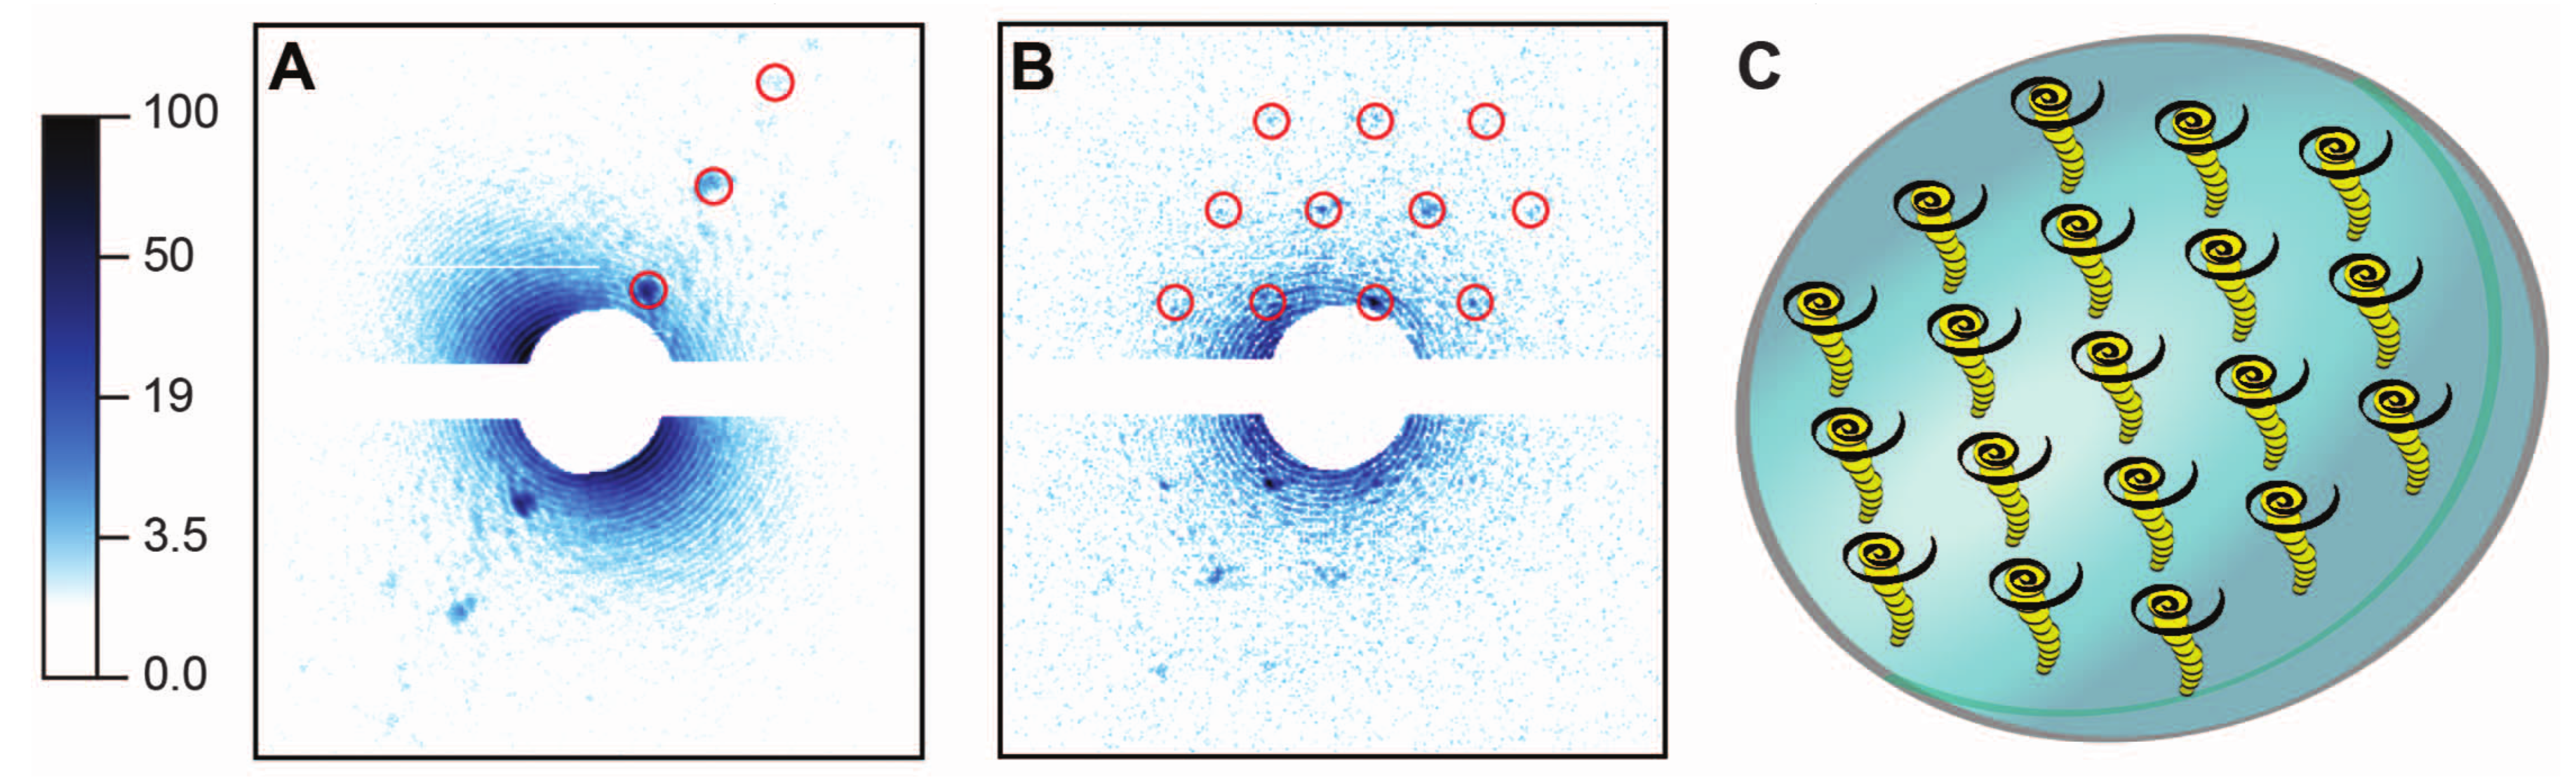
\includegraphics[width=\textwidth]{vortex-array}
			\caption{He droplets doped with Xe atoms. (A and B) X-ray diffraction images of doped droplets, displayed in a logarithmic intensity scale. (C) Droplet and embedded Xe clusters. Images in (A) and (B) correspond to tilted and parallel alignments of the vortex axes with respect to the incident x-ray beam, respectively.}
			\label{fig:vortex-array}
		\end{center}
	\end{figure}
	
%	\section{Head-on collisions}
%		\lettrine[lines=3,findent=3pt,nindent=0pt]{I}{t} is well known that helium drops readily capture foreign atoms and molecules[1], and this ability has had a considerable influence on the chemistry and physics of these systems[2]. Among the studies carried out in the past on atom-drop collisions, let us mention those aiming at experimentally determining the density profiles of large $^4$He and $^3$He droplets from the scattering of Ar and Kr atoms off helium droplets, which have been analysed within density functional theory (DFT)[3,4]; the microscopic simulation of the scattering of 3He and 4He atoms from inhomogeneous liquid helium systems[5,6]; and an earlier theoretical work on the scattering of 4He atoms from 4He droplets within a liquid drop plus optical model approach[7].\\
%
%		Very recently, time-dependent density functional theory (TDDFT) has been used to address the capture of Cs or Ne atoms by $^4$He nanodroplets[8,9]. The Cs capture was treated fully three dimensionally with the Cs atom described as a classical particle, whereas for the Ne capture study the Ne atom was described quantum mechanically, but the description was strictly one dimension.\\
%
%		Motivated by recent experiments that use Xe atoms to visualise vortex arrays in very large helium droplets[10,11], we present here a first step toward the description of the capture of Xe atoms by helium droplets, namely head-on collisions of Xe atoms against a $^4$He$_{1000}$ droplet. A discussion on the dynamic capture of Xe atoms by droplets hosting vortex lines and vortex arrays will be provided by a forthcoming study combining DFT simulation of vortex arrays as in Refs.[12,13] for helium nanocylinders and nanodroplets and collision with Xe atoms as in this work. Whenever possible, the results for Xe, a heliophilic atom, are contrasted with results for Cs, a heliophobic atom with similar mass.
%
%	\section{Capture by quantised vortices}
%		\lettrine[lines=3,findent=3pt,nindent=0pt]{I}{t} is well established that helium droplets can readily capture in their interior almost any atom or molecule interacting with them, as first shown for the case of Ne atoms[1], with the notable exception of alkali[2] and some alkaline-earth[3] atoms. This property, together with the extremely low temperature (T) achieved in helium droplets -- of the order of 0.4 K -- makes them the perfect ultracold and inert environment for hosting and studying isolated atoms and molecules, which is at the basis of current applications of helium droplets for spectroscopic studies of atoms and molecules. Besides, the superfluid nature of helium facilitates binary encounters of atoms/molecules in the bulk of the droplet while absorbing the energy released upon recombination, making possible chemical reactions which would not otherwise occur in the gas phase. These unique properties of helium droplets have had a huge impact on their study[4-8].\\
%
%		The pickup of Ar, Kr and Xe atoms in the gas phase by $^4$He$_N$ droplets with $N>10^3$ atoms produced by nozzle beam expansions was described about twenty years ago by Toennies and coworkers[9]. In these experiments, the droplets in the helium beam were deflected by impacting with a secondary beam made of rare gas atoms.\\
%
%		Recently, a technique has been introduced to determine the size of large He droplets ($N>10^5$). It is based on the attenuation of a continuous droplet beam through collisions with Ar atoms at room temperature[10]. The pickup chamber of the droplet beam apparatus is filled with argon gas and the helium droplets experience multiple, isotropic collisions with the Ar atoms on their way towards the detection chamber. Large helium droplets could also be doped in this way. This method, using Xe atoms, has been instrumental for detecting and imaging quantised vortex arrays in helium droplets[11,12]. Xe atoms were used in these experiments because of their large sensitivity to the X-ray coherent diffractive imaging employed to detect them within the helium droplets. Experiments with large superfluid helium droplets are reviewed in a recent publication[14].\\
%
%		The impurity-droplet interaction in the presence of vortices is also relevant as the first stage of a more complex process leading to the formation of nanowires, see e.g. ref. 15-18. Long filaments made of micrometer-sized solid hydrogen particles trapped on quantised vortex cores were used to directly image the vortex reconnection between quantised vortices in superfluid helium[19].\\
%
%		The impact and capture of impurities interacting with pure helium droplets have been addressed recently within time-dependent density functional theory (TDDFT). Real-time simulations have been carried out for heliophobic[20] (Cs) and heliophilic[21] (Ne) atoms. In addition to the TDDFT equation for $^4$He, heavy impurities are treated as classical particles using Newton's equation of motion, whereas a time-dependent Schr\"{o}dinger equation has been used in the case of light impurities within the mean field model[21,22]. A comparison between the results for head-on collisions of Cs and Xe atoms -- heliophobic and heliophilic atoms of similar mass -- has been presented in ref. 23.\\
%
%		In this work, we present the results obtained within TDDFT for the collision and capture of Xe and Ar atoms by a $^4$He$_{1000}$ droplet at different kinetic energies and impact parameters. Special attention is paid to the time-dependent interaction of Xe and Ar atoms with helium nanodroplets hosting vortex lines, and to the effect of multi-doped vortex arrays in large helium droplets.\\
%
%		Due to the heavy computational cost of the TDDFT simulations presented here, we address only a few facets of the capture process that we consider of experimental relevance rather than carrying out a systematic study of the process. In particular:
%		\begin{itemize}
%			\item We study the capture of Xe atoms by a $^4$He nanodroplet, both for head-on collisions and for different impact parameters, with velocities ranging from thermal values up to several hundred m/s. The results of peripheral collisions with different values of the impact parameter are used to estimate the cross section for the Xe capture.
%			\item We study how a Xe atom dynamically interacts with a droplet hosting a vortex line, under different initial conditions resulting in different velocity regimes of the impurity as it collides with the vortex core: 
%			\begin{enumerate}
%				\item[i)] a Xe atom initially at rest on the droplet surface and sinking under the effect of solvation forces
%				\item[ii)] a head-on collision of a moving Xe or Ar atom against the $^4$He nanodroplet.	
%			\end{enumerate}
%			\item We study the stationary state of a large $^4$He$_{15000}$ droplet hosting a ring of six vortex lines, doped with Ar atoms completely filling all six vortex cores. This is the simplest system that mimics those experimentally described in ref. 11, where doped vortex arrays embedded in rotating $^4$He microdroplets have been imaged.
%		\end{itemize}
%
%		Multimedia materials accompany this paper, showing the real-time dynamics of several impact/capture processes described here. These materials are presented in the ESI document. They constitute an important part of this work, since often it is only by viewing how a complex microscopic process unfolds in real-time that one can catch important physical details which would otherwise escape in a written account.